\documentclass[]{standalone}

\usepackage{graphicx}
\usepackage[linesnumbered,ruled,vlined]{algorithm2e}
\usepackage{color,soul}
\usepackage[utf8]{inputenc}
\usepackage[T1]{fontenc}
\usepackage{textcomp}
\usepackage{amsmath, amssymb}
\usepackage{caption}
\usepackage{listings}

% figure support
\usepackage{tikz}
\usetikzlibrary{calc}
\usepackage{import}
\usepackage{xifthen}
\pdfminorversion=7
\usepackage{pdfpages}
\usepackage{transparent}
\usepackage[hidelinks]{hyperref}

\pdfsuppresswarningpagegroup=1

\begin{document}

		
		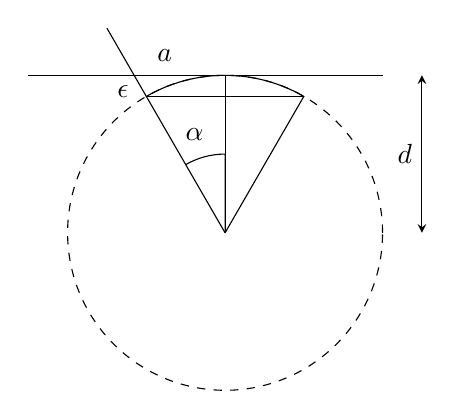
\begin{tikzpicture}[>=stealth]
			\draw (0,0) -- (0,2);
			\draw (-2.5,2) -- (2,2);
			\draw (0,0) -- ++ (120:3);
			\draw (0,0) -- ++ (60:2) arc (60:120:2);
			\draw[dashed] (0,0) circle[radius=2];
			\draw (0,0) -- ++ (90:1) arc (90:120:1);
			\draw (0,0) ++ (60:2) -- ++ (-2,0);
			\node[anchor=east] (alpha) at(-0.15,1.25) {$\alpha$};
			\node[anchor=east] (epsilon) at(-1.1,1.8) {$\epsilon$};
			\draw[<->] (2.5,2)--(2.5,0);
			\node[anchor=east] (d) at (+2.5, 1) {$d$};
			\node[anchor=east] (a) at (-0.55, 2.25) {$a$};
			\node[] () at (2.5,0) {$$};
			
		\end{tikzpicture}
		
		
\end{document}
